% ERA-Großpraktikums: Benutzeranleitung -- Features

\section{Features}

\subsection*{Überblick}

\todo[inline]{Bild mit nummerierten Komponenten einfügen.}

\begin{enumerate}
\item \textbf{Editor:} Hier wird der Assemblercode geschrieben, der vom
Simulator assembliert und ausgeführt werden soll.
\item \textbf{Toolbar:} Enthält Knöpfe zur Ausführung des Assemblerprogramms.
\item \textbf{Tabbar:} Zeigt aktuell geöffnete Projekte an.
\item \textbf{Register:} Zeigt Prozessorregister und erlaubt Bearbeitung der
Registerwerte.
\item \textbf{Speicher:} Zeigt Hauptspeicherinhalt und erlaubt Bearbeitung
einzelner Speicherzellen.
\item \textbf{Hilfe:} Zeigt Hilfestellungen zur aktiven Zeile im Editor an.
\item \textbf{Output:} Bietet Auswahl an Ausgabegeräten, die über den Speicher
angesteuert werden können.
\item \textbf{Input:} Bietet Auswahl an Eingabegeräten, die Benutzereingaben
empfangen und kodiert in den Speicher schreiben.
\item \textbf{Snapshots:} Erlaubt das Erzeugen und Laden von Schnappschüssen
des Prozessorzustands (Register- und Speicherinhalt).
\end{enumerate}

% Ich schlage eine Teilung der einzelnen Features nach Projektverwaltung(Laden, Speichern, Snapshots), Erstellen von Programmen (Editor, Hilfetexte), Ausführung von Programmen(Ausfühmodi, Breakpoints), Interaktion mit laufenden Programmen (Input/Output-Components) und sonstiges vor

\subsection{Projekt}

\subsubsection{Projekt erstellen}
\label{sec:project_creation}

\begin{figure}[ht]
	\centering
  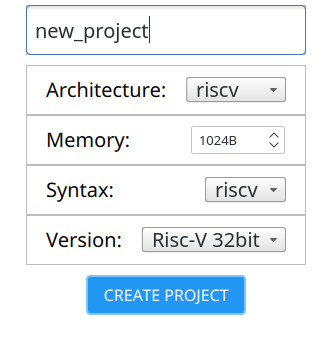
\includegraphics[scale=1]{Images/create_new_project}
	\caption{Erstellen eines neuen Projekts}
	\label{Project_Creation}
\end{figure}

Nach dem Start des Programms erscheint ein Fenster in dem ein neues Projekt
erstellt werden kann. Sind bereits andere Projekte geöffnet so kann ein weiteres
über den Plus-Knopf der Projekt-Tabbar, über die Menüleiste oder den
Tastaturbefehl \texttt{Strg-N} (\texttt{Cmd-N} auf macOS) angelegt werden.

Neben dem Projektnamen muss dafür auch die zu simulierende Architektur angegeben
werden. Diese beinflusst im Wesentlichen, welche
Assembler-Instruktionen und Register zur Verfügung stehen.

Darüber hinaus kann die Hauptspeichergröße frei gewählt werden, wobei der Wert
zwischen 4 und 1.048.576 Byte liegen muss.

Mit der Wahl der Syntax wird die Art und Weise, wie Assembler-Instruktionen
geschrieben werden, festgelegt. Eine Syntax unterscheidet sich von der anderen
beispielsweise in der Art, wie der Immediate-Teil einer Instruktion geschrieben
wird. Der verfügbare Instruktionssatz selbst wird dadurch nicht beeinflusst.

Manche Architekturen stehen in verschiedenen Versionen zur Verfügung. RISC-V
etwa kann in einer 32 Bit Variante oder in einer 64 Bit Variante verwendet
werden, was sich hauptsächlich auf die Länge der Register bezieht.


\subsubsection{Speichern/Laden}

Der Simulator unterstützt nicht das Speichern ganzer Projekte, sondern
ermöglicht es stattdessen, den Assemblercode als Datei zu speichern, während der
Prozessorzustand (Register- und Speicherinhalt) getrennt als Snapshot
gespeichert werden können. Dies ermöglicht es, ein und denselben Snapshot in
mehreren Projekten zu verwenden.

Um den Assemblercode eines Projekts zu speichern wählt man in der Menüleiste die
Option ``Editor'' $\rightarrow$ ``Save File'' aus und gibt einen Speicherort für
die Datei an.

Möchte man gespeicherten Assemblercode laden, so erstellt man zunächst ein neues
Projekt und wählt dann über ``Editor'' $\rightarrow$ ``Open File'' die
gewünschte Datei aus, deren Inhalt darauf im Editor erscheint.

Um den Inhalt der Register und des Speichers persistent zu speichern, werden wie
bereits erwähnt, Snapshots verwendet, deren Benutzung im folgenden Abschnitt
erklärt wird.

\subsubsection{Snapshots}

Snapshots sind, wie der Name bereits nahelegt, Schnappschüsse des
Prozessorzustands, also der Register- und Speicherinhalte. Sie eigenen sich
dazu, die Werte von Registern und Speicher automatisch in einen festgelegten
Zustand zu bringen. Hat man beispielsweise ein Assemblerprogramm, dass auf
bestimmten Ausgangswerten in Registern oder Speicher basiert, so kann man diese
Werte zunächst manuell eintragen und dann einen Snapshot des aktuellen Zustands
anlegen. Wurden die Inhalte von Registern und Speicher anschließend etwa durch
die Programmausführung geändert, so kann man durch Laden des Snapshots ganz
einfach wieder zum Ausgangszustand zurückkehren.

Ein Snapshot wird über den Plus-Button in der Snapshot-Komponente oder die
Menüleiste (``Project'' $\rightarrow$ ``Save Snapshot'') erstellt und mit einem
eindeutigen Namen versehen. Die Werte, die zum Zeitpunkt des Schnappschusses in
den Registern und im Speicher geschrieben stehen, werden dadurch im Snapshot
gespeichert. Anschließend können die Register- und Speicherinhalte nach Belieben
verändert werden, egal ob durch Drücken des Reset-Buttons, manuelles Ändern der
Werte oder Ausführen eines Assemblerprogramms, das den Prozessorzustand
verändert. Um einen Snapshot zu laden, wird einfach auf den zugehörigen Eintrag
in der Snapshot-Komponente gedrückt.

\begin{warningblock}
Durch Laden eines Snapshots wird der aktuelle Prozessorzustand überschrieben.
Soll dieser also nicht verloren geht, muss vorher ein weiterer Snapshot erstellt
werden.
\end{warningblock}

Snapshots werden projektübergreifend abgelegt, ein Snapshot der in einem Projekt
erstellt wurde, kann im Allgemeinen auch in einem anderen Projekt geladen
werden. Es gilt allerdings zu beachten, dass ein Snapshot an eine bestimmte
Architektur und sogar an eine bestimmte Version einer Architektur (siehe
\ref{sec:project_creation} ``Projekt erstellen'') gebunden ist, da sich die etwa
die Länge der Register je nach Architektur-Version unterscheiden können. Ein
Snapshot der zum Beispiel für ein Projekt der RISC-V 32Bit Version erstellt
wurde, kann nicht in einem Projekt mit RISC-V 64Bit Version geladen werden.

\subsection{Erstellen von Programmen}

\subsubsection{Editor}
\label{sec:Editor}

Im Editor wird der Assemblercode verfasst, der vom Simulator assembliert und
ausgeführt werden kann. Durch Syntax-Highlighting werden bestimmte
Code-Fragmente, wie Kommentare, Instruktionen, Registernamen oder Immediate-Werte,
farblich gekennzeichnet.

Während des Schreibens erscheint unterhalb der aktuellen Zeile, in der sich der
Cursor befindet, ein Fragezeichenfeld, über das bei Bedarf die
Befehlsdokumentation der gegebenenfalls unvollständigen Assemblerinstruktion
angezeigt werden kann.

Makrodefinition werden wie alle anderen Instruktionen an jedwede Stelle ins
Code-Dokument geschrieben und können anschließend beliebig oft aufgerufen
werden. Jeder Makroaufruf kann außerdem über einen dreieckige Button in
der Editor-Seitenleiste aufgeklappt werden, wodurch die Makroerweiterung
unterhalb des eigentlichen Makroaufrufs eingeblendet wird. Makroparameter werden
dabei durch die konkreten Argumente des Aufrufs ersetzt. Durch das Anzeigen der
Makroerweiterung direkt beim Makroaufruf wird verdeutlicht, dass es sich bei
Makroaufrufen nicht um einen Funktionsaufruf handelt, sondern um eine
Text-Ersetzung, die vom Assemblierer durchgeführt wird.

Wird das Code-Dokument verändert, so werden alle Makroerweiterungen wieder
eingeklappt.

Fehlermeldungen, Warnungen und Hinweise werden im Editor direkt in der
betroffenen Zeile eingeblendet. Gehören mehrere Meldungen zu einer einzelnen
Zeile, so werden diese untereinander angezeigt. Durch Klicken auf das zugehörige
Meldungssymbol in der Editor-Seitenleiste, können alle Meldungen einer Zeile
ein- und ausgeblendet werden.

\begin{figure}[ht]
	\centering
  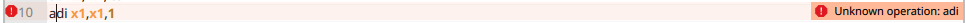
\includegraphics[width=\textwidth]{Images/Editor_error}
	\caption{Ein Fehler im Texteditor}
	\label{Editor_Error}
\end{figure}

Des Weiteren besteht die Möglichkeit im Editor zu zoomen. Dazu wird bei
gleichzeitigem Drücken der Steurungstaste (Cmd-Taste bei Mac-Computern)
gescrollt.

\begin{figure}[ht]
	\centering
  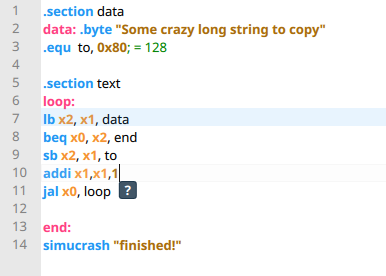
\includegraphics[scale=1]{Images/Editor}
	\caption{der Programmeditor}
	\label{Editor}
\end{figure}


\begin{figure}[ht]
	\centering
  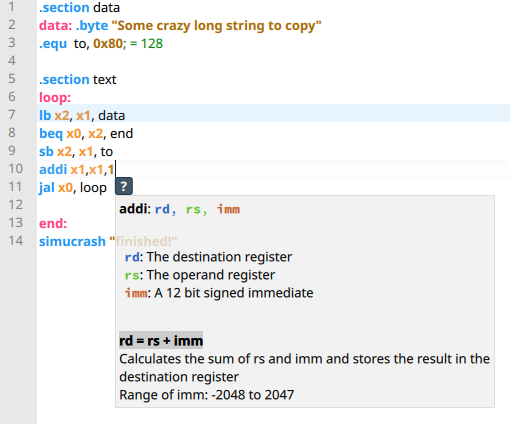
\includegraphics[scale=0.7]{Images/Editor_help}
	\caption{die Inline-Hilfe im Texteditor}
	\label{Editor_Help}
\end{figure}




\subsubsection{Hilfetextkomponente}
\label{help-component}
%\todo[inline]{Was wird angezeigt, zu welchem Befehl (Zeile!), wann (nach dem Parsen)}

Die Hilfetextkomponente zeigt die Befehlsdokumentation des Befehls der aktuellen
Zeile an und ergänzt damit das Hilfefenster, das bei Bedarf direkt im Editor
angezeigt werden kann (siehe \ref{sec:Editor} ``Editor''). Die
Hilfetextkomponente bezieht sich immer auf den Befehl der Zeile, in der sich der
Cursor befindet. Gegebenenfalls ist die Anzeige eines Hilfetextes leicht
verzögert, da der aktuelle Code erst neu geparst werden muss.


\subsection{Ausführung von Programmen}

\subsubsection{Ausführungsmodi}

\begin{figure}[ht]
	\centering
  
\includegraphics[scale=1]{Images/Toolbar}
	\caption{Die Toolbar zum kontrollieren der Programmausführung}
	\label{Toolbar}
\end{figure}

Der Simulator verfügt über drei verschiedene Ausführungsmodi. Die Zeile, an der
die Ausführung begonnen wird, ist im Editor stets farblich hervorgehoben.

Der erste Modus (erster Button von links in Abbildung \ref{Toolbar}) führt das
ganze Programm komplett ab der hervorgehobenen Zeile aus.

Möchte man die Ausführung dabei beenden, beispielsweise wegen einer
Endlosschleife, so klickt man auf den Stopp-Button (vierter Button von links).

Darüber hinaus gibt es die Möglichkeit nur die aktuelle Zeile auszuführen, also
Schritt für Schritt (zweiter Button von links). Hierbei werden die geänderten
Werte in den Registern hervorgehoben, was in anderen Modi nicht der Fall ist.

Im letzten Ausführungsmodus wird das Programm bis zum nächsten Breakpoint
ausgeführt (dritter Button von links). Einen neuen Breakpoint erstellt man,
indem man in der Seitenleiste auf den Bereich neben der zugehörigen Zeile
klickt. Durch erneutes Klicken auf den Breakpoint wird dieser wieder entfernt.

\todo[inline]{Ggf. Bild von Breakpoint}

Drückt man nach beendeter oder unterbrochener Ausführung auf den Reset-Button (erster
Button von rechts), so wird der Zeiger für die nächste auszuführende Zeile wieder
an den Anfang des Programms gesetzt und die Register- und Speicherinhalte zurückgesetzt.


\subsubsection{Registerkomponente}
Die Registerkomponente zeigt die
Prozessorregister an und ermöglicht es, deren Werte manuell zu verändern. Jedes
Register besteht aus einem Registertitel, mit dem es in der Regel auch im
Assemblercode referenziert werden kann, sowie dem zugehörigem Registerinhalt.

Der Registerinhalt kann je nach Art des Registers unterschiedlich formatiert
werden. Allzweckregistern stehen die Formate \textit{Binär},
\textit{Hexadezimal}, \textit{Dezimal (vorzeichenbehaftet)} und \textit{Dezimal
(nicht vorzeichenbehaftet)} zur Verfügung. Ein-Bit Flag-Register können außerdem
als Checkbox angezeigt werden. Das aktuelle Format des Registers wird rechts vom
Registertextfeld über den Formatindikator angezeigt (\textit{S}: signed decimal,
\textit{U}: unsigned decimal, \textit{H}: hexadecimal, \textit{B}: binary,
\textit{F}: flag). Zum Anpassen des Formats kann entweder auf den
Formatindikator geklickt werden und die passende Optionen ausgewählt werden oder
gescrollt werden, während sich der Mauszeiger über dem Formatindikator befindet.
Beachten Sie, dass für ein Register unter Umständen nicht alle Format-Optionen
zur Verfügung stehen --- so kann der Programmzähler etwa nicht im Dezimal-Format
angezeigt werden.

Um den Wert eines Registers manuell zu ändern, wird der Text im Textfeld
bearbeitet und die Eingabe mit Enter bestätigt. Auf die Einhaltung der
Formatierung muss nicht geachtet werden. Nach Bestätigung der Eingabe wird der
Registerwert automatisch der aktuellen Einstellung entsprechend formatiert. Ist
zudem ein eingegebener Wert zu lang um in der im Register gegebenen Größe gespeichert
werden zu können, werden die höherwertigen überschüssigen Zeichen entfernt.
Gleichermaßen wird der Registerinhalt durch höherwertige Nullen auf seine
Maximalgröße aufgefüllt. Ungültige Zeichen werden automatisch entfernt.

Über das Einstellungsmenü der Registerkomponente (erreichbar über die Kopfzeile
der Komponente oder durch Rechtsklick) können alle Register auf einmal
formatiert werden. Steht das gewählt Format für ein Register nicht zur Verfügung
(bspw. Dezimal für den Programmzähler), so behält dieses seine ursprüngliche
Formatierung bei.

Einige Register können je nach Architektur fest verdrahtet sein und können
deshalb weder über eine Assemblerinstruktion noch manuell geändert werden. Die
Textfelder dieser Register sind deaktiviert.

Führt man eine einzelne Zeile aus, die den Wert eines Registers ändert, so wird
dieses farblich hinterlegt, damit die Änderung schneller nachvollzogen werden
kann.


\subsubsection{Speicherkomponente}
Der Hauptspeicher spielt bei allen Programmen eine sehr wichtige Rolle. Dort
sind sowohl der assemblierte Programmcode, der Callstack, als auch Daten zum
Arbeiten hinterlegt. Der Speicher ist dabei in Zellen unterteilt, die in der
Regel 1 Byte groß sind. Auch der Simulator hat natürlich einen solchen RAM, der
sich flexibel an die Bedürfnisse des Nutzers anpassen lässt.

\begin{figure}[ht]
	\centering
  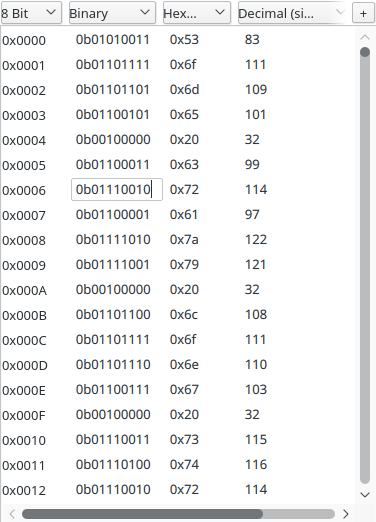
\includegraphics[scale=1]{Images/Memory}
	\caption{der Programmspeicher - RAM}
	\label{Memory}
\end{figure}

Um den Inhalt des Speichers auf einen Blick erfassen zu können, stehen
verschieden Einstellungen in der Kopfzeile zur Verfügung:\\ In der ersten Spalte
stehen immer die Adressen der Speicherzellen. Bei großen Datenmengen ist es
manchmal wünschenswert mehr als nur 1 Byte pro Zeile angezeigt zu bekommen.
Deshalb kann im Menü oberhalb dieser Spalte die angezeigte Größe der
Speicherzellen eingestellt werden. Standardmäßig stehen hier $8\, Bit$, $16\,
Bit$, $32\, Bit$ und $64\, Bit$ zur Auswahl. Dabei wird aber die die
architekturbedingte Größe der Speicherzellen nicht beeinflusst; es werden
stattdessen mehrere Speicherzellen pro Zeile dargestellt. Deshalb ändert sich
die angezeigte Adressierung entsprechend.\\ Des Weiteren stehen mehrere
Anzeigeformate für den Inhalt zur Verfügung, welche jeweils oberhalb einer
angezeigten Spalte ausgewählt werden können. Dabei stehen standardmäßig
\textit{Binär}, \textit{Hexadezimal}, \textit{Dezimal (nicht vorzeichenbehaftet/unsigned))} und \textit{Dezimal (vorzeichenbehaftet/signed)} zur Verfügung. Letzteres kann den Speicherinhalt
auch als negative Zahl interpretieren bzw. auch negative Eingaben entgegen
nehmen. \\

\begin{figure}[ht]
	\centering
  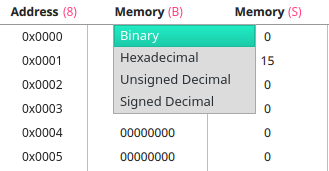
\includegraphics[scale=1]{Images/Memory_Representation}
	\caption{Die Auswahl der Speicherrepräsentationen}
	\label{Memory_Respresentations}
\end{figure}

Außerdem können die Inhalte der Speicherzellen nebeneinander gleichzeitig in
verschiedenen Formaten repräsentiert werden. Dazu einfach auf das ``\texttt{+}''
in der rechten oberen Ecke klicken. Daraufhin erscheint eine neue Spalte im
Speicher, bei der auch wieder das Format ausgewählt werden kann. Um eine Spalte
wieder zu entfernen, muss im Kontextmenü im Spaltenheader der Eintrag
``\texttt{remove...}'' ausgewählt werden.

\begin{warningblock}
Bei einer ungültigen Eingabe wird die Zahl bestmöglich interpretiert und
anstelle des eingegebenen Wertes an die Speicherstelle geschrieben. Dazu zählt
auch die Eingabe zu großer Zahlen. Die Ersetzung erfolgt sofort.
\end{warningblock}

Eine Speicherzelle kann außerdem als read-only markiert sein. 
Dies kann passieren, wenn die Speicherzelle einen Teil des ausführbaren 
Programmcodes enthält. 
Das Betriebssystem markiert bestimmte Bereiche des Speichers als 
schreibgeschützt, um selbstmodifizierenden Code zu verhindern.
Dieser Schutz ist sehr wichtig um Schadprogramme zu verhindern.
Auch der Simulator markiert die Speicherzellen, den den assemblierten Code
enthält, als schreibgeschützt. Ein kleines Symbol in der rechten oberen Ecke
der Adresse zeigt dies an.

\begin{figure}[ht]
	\centering
  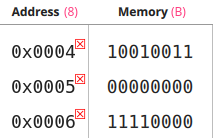
\includegraphics[scale=1]{Images/Memory_writeprotected}
	\caption{Eine schreibgeschützte Speicherzelle}
	\label{Memory_writeprotected}
\end{figure}


\subsection{Interaktion mit laufenden Programmen}
%\todo[inline]{Hier sollte (für alle Komponenten ja gleich) die Einstellungsmöglichkeiten (Zahnrad-knopf) und welches Symbol welche Komponente bedeutet}

Der Simulator unterstützt eine Reihe von Ein- und Ausgabekomponenten, die im
Folgenden erläutert werden. Eine Eingabekomponente nimmt dabei Eingaben des
Nutzers über die Benutzeroberfläche des Simulators entgegen, während
Ausgabekomponenten Zahlenwerte graphisch darstellen.

Die Kommunikation mit den Ein- und Ausgabekomponenten erfolgt über den Speicher.
Für Eingabekomponenten lässt sich eine Adresse im Speicher, die sogenannte
\textit{Memory Source Address} angeben, an die jegliche eingelesene Werte
geschrieben werden. Analog gibt es auch für Ausgabekomponenten eine
\textit{Memory Source Address}, die angibt, von welcher Stelle im Speicher an
Daten von der Ausgabekomponente ausgelesen und graphisch interpretiert werden.
Da auch Ausgabekomponenten oftmals Benutzereingaben zulassen, werden gleichfalls
Daten in den Speicher geschrieben, natürlich an die gleiche \textit{Memory Source
Address}, die auch zum Einlesen verwendet wird.

Die \textit{Memory Source Address}, sowie gegebenenfalls weitere Optionen, können
über das Einstellungsmenü jeder Ein- und Ausgabekomponente einzeln festgelegt
werden. Man erreicht das Menü über den Komponenten-Header, der am Kopf einer
Komponente eingeblendet wird, wenn man den Mauszeiger darüberbewegt. Ein Klick
auf den Zahnradbutton (
\includegraphics[scale=0.22]{Images/SettingsIcon}) öffnet
das Einstellungsfenster.

\subsubsection{Eingabe -- Tastatur}

Die Tastatur-Eingabekomponente fängt einzelne Tastatureingaben ab und schreibt
eine Kodierung, die der gedrückten Taste entspricht, in den Speicher.

Ein Klick auf das Rechteck im Zentrum der Komponente startet die Eingabe. In
diesem Zustand werden alles Tastatureingaben abgefangen und in den Speicher
geschrieben. Die Adresse im Speicher, an die die Kodierung geschrieben wird, ist
durch die \textit{Memory Source Address} festgelegt. Diese bleibt im Laufe der
Eingaben konstant, das heißt ein neues Tastensignal überschreibt die alte
Kodierung im Speicher. Erneutes Klicken auf das Rechteck beendet die Eingabe.

Eine Tastenkodierung ist 4 Byte lang. Eine Übersicht über die unterstützten
Tasten und die zugehörige Kodierung, die in den Speicher geschrieben wird, bietet
Tabelle \ref{tab:keys}.

\begin{figure}
	\centering
	\begin{tabular}{ll}
	\textbf{Taste} & \textbf{Wert} \\
	\hline
	Escape & 0x01000000 \\
	Return & 0x01000004 \\
	eft & 0x01000013 \\
	Up & 0x01000014 \\
	Right & 0x01000015 \\
	Down & 0x01000016 \\
	Space & 0x00000020 \\
	Tab & 0x01000001 \\
	Backspace & 0x01000003 \\
	Shift & 0x01000020 \\
	Plus & 0x0000002b \\
	Comma & 0x0000002c \\
	Minus & 0x0000002d \\
	Period & 0x0000002e \\
	Slash & 0x0000002f \\
	0 & 0x00000030 \\
	... & ... \\
	9 & 0x00000039 \\
	A & 0x00000041 \\
	... & ... \\
	Z & 0x0000005a \\
\end{tabular}
	\caption{Liste der wichtigsten Tasten und zugehöriger Kodierung, die in den
	Speicher geschrieben wird.\newline Quelle und vollständige Tabelle:
	\url{http://doc.qt.io/qt-4.8/qt.html\#Key-enum}}
	\label{tab:keys}
\end{figure}

Über das Einstellungsmenü der Komponente kann die \textit{Memory Source Address}
festgelegt werden, also die Adresse im Speicher, an die die kodierte
Tastatureingabe geschrieben wird.

\begin{figure}[ht]
	\centering
	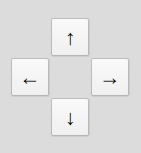
\includegraphics[width=0.2\textwidth]{Images/Joystick}
	\caption{Eingabe über Tastatur}
	\label{Joystick}
\end{figure}


\subsubsection{Eingabe -- Mausklick}
%\todo[inline]{welche werte werden geschrieben, Reihenfolge?}
Die Mausklick-Eingabekomponente liest Mausklicks des Benutzers über einen
Klick-Bereich ein und schreibt die x- und y-Koordinate des Klicks relativ zum
Klick-Bereich in den Speicher. Der Klick-Bereich deckt ein Koordinatensystem von
$0$ bis $255$ in beiden Dimensionen ab, unabhängig von der absoluten Größe des
Bereichs. Der Koordinatenursprung liegt in der linken oberen Ecke des
Klick-Bereichs. Die Koordinate eines Klicks ergibt sich relativ zur Länge des
Rechtecks in der jeweiligen Dimension. Ist das Rechteck 100 Pixel breit und wird
auf das zwanzigste Pixel geklickt, so ergibt sich die x-Koordinate $20 / 100
\cdot 255 = 51$. Die Koordinaten werden stets abgerundet.

Die eingelesenen Werte werden an die \textit{Memory Source Address} in
den Speicher geschrieben. Sowohl die x- als auch die y-Koordinate werden als
8-Bit-Werte in den Speicher geschrieben, wobei die x-Koordinate vor der
y-Koordinate steht.

\begin{figure}[ht]
	\centering
	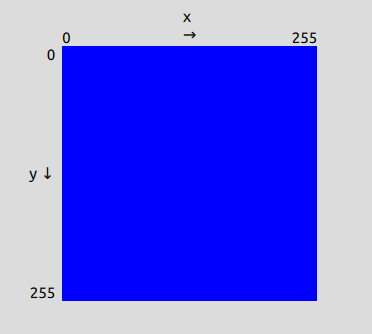
\includegraphics[width=0.3\textwidth]{Images/MouseArea}
	\caption{Eingabe mit Mausklick}
	\label{MouseArea}
\end{figure}

\subsubsection{Ausgabe -- Lichtbandanzeige}

Die Lichtbandanzeige dient hauptsächlich zur Anzeige verschiedener Arten von
Fortschrittsbalken. Sie besteht aus mehreren einzelnen Leuchtkomponenten, der
Anzahl im Einstellungsmenü der Anzeige definiert werden kann. Jede
Leuchtkomponente kann durch ein Bit im Speicher an der richtigen Adresse
angesteuert werden. Eine \texttt{1} bedeutet dabei, dass das Segment leuchtet;
also farbig dargestellt wird. Bei einer \texttt{0} wird die Fläche in Grau
dargestellt. Die Bits sind im Speicher an direkt aufeinanderfolgenden Stellen zu
setzen. Ein Byte kann somit eine Leuchtbandanzeige aus 8 Elemente komplett
ansteuern. Dabei ist der Nutzer natürlich nicht darauf beschränkt eine
Fortschrittsanzeige von links nach rechts aufzubauen, sondern kann jede Fläche
unabhängig voneinander ein und ausschalten. Als Alternative kann man auch mit
der Maus auf ein Leuchtfeld klicken, um es an- bzw. auszuschalten. Der
Speicherinhalt an der entsprechenden Adresse wird dadurch entsprechend
geändert.\\


\begin{figure}[ht]
	\centering
  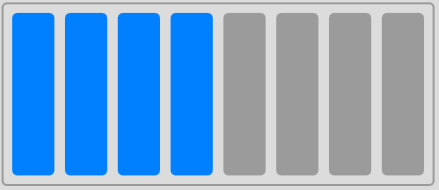
\includegraphics[width=0.8\textwidth]{Images/Lightstrip}
	\caption{Leuchtbandanzeige}
	\label{Lightstrip}
\end{figure}

Ein besonderes Feature ist dabei die individuelle Gestaltung der
Lichtbandanzeige. Bei einem Rechtsklick auf ein Leuchtelement öffnet sich ein
Farbwahldialog, wo die Leuchtfarbe des Segments gewählt werden kann.

\begin{figure}[ht]
	\centering
  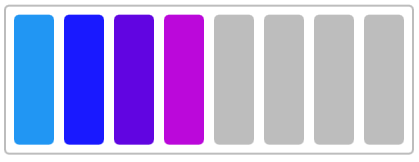
\includegraphics[width=0.8\textwidth]{Images/Lightstrip_colors}
	\caption{Leuchtbandanzeige mit verschiedenen Farben}
	\label{Lightstrip_Colors}
\end{figure}


\subsubsection{Ausgabe -- 7-Segmentanzeige}
Die sogenannte 7-Segment Anzeige ist eine einfache alphanumerische Ausgabe, wie
sie häufig bei kleinen digitalen Geräten zum Einsatz kommt. Die Anzeige besteht, wie
der Name schon sagt, aus 7 Strichen, die unabhängig voneinander zum Leuchten
gebracht werden können.

\begin{figure}[ht]
	\centering
  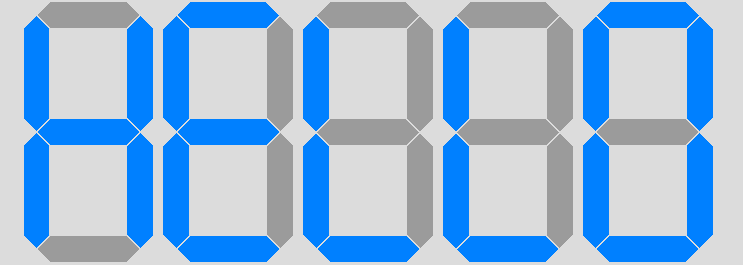
\includegraphics[width=0.8\textwidth]{Images/7-Segment_Hello}
	\caption{Die 7-Segment Anzeige im Simulator}
	\label{7-Segment}
\end{figure}

Jedes dieser Segmente wird durch ein einzelnes Bit angesteuert. Dabei bedeutet $1$, dass das Segment leuchten soll und $0$ entsprechend, dass es nicht leuchten soll.
Pro Zeichen wird somit ein Byte zum Ansteuern benötigt, wobei das höchstwertige Bit in der Regel ignoriert wird.

Wenn man die Maus im Simulator über ein Zeichen bewegt, erscheint dort die Reihenfolge, in der die Bits den einzelnen Segmenten zugeordnet sind.

\begin{figure}[ht]
	\centering
  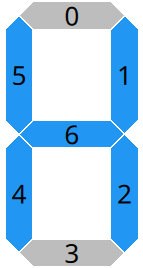
\includegraphics[width=0.2\textwidth]{Images/7-Segment_Hover}
	\caption{Die Reihenfolge der Bits}
	\label{7-Segment_Hover}
\end{figure}

Es können auch gleichzeitig mehrere Zeichen angesteuert werden. Die einzelnen
Bytes für jedes Zeichen stehen dann im Speicher an aufeinanderfolgenden
Adressen. Dabei muss aber darauf geachtet werden, dass die Reihenfolge genau
umgedreht ist. Das Zeichen am rechten Rand steht somit an der ersten Adresse im
Speicher, danach folgt das vorletzte usw.

\begin{warningblock}
Reihenfolge der Zeichen: Die Ansteuerung der Zeichen geschieht (wie im Zahlensystem) von rechts nach links.
\end{warningblock}

Ein kleines Beispiel verdeutlicht dies wohl am besten.

\begin{exampleblock}{HELLO}
	Für das oben gezeigte \texttt{HELLO} wäre also folgende Ansteuerung nötig:\\
	\begin{tabular}{llll}
	0x3f & 0b00111111 & & \texttt{O}\\
	0x38 & 0b00111000 & & \texttt{L}\\
	0x38 & 0b00111000 & & \texttt{L}\\
	0x79 & 0b01111001 & & \texttt{E}\\
	0x76 & 0b01110110 & & \texttt{H}\\
	\end{tabular}
\end{exampleblock}

Falls man sich den Umweg über die Ansteuerung über Speicheradressen sparen möchte,
kann man die einzelnen Leuchtsegmente auch durch einen Klick mit der linken Maustaste aktivieren bzw. deaktivieren.

Für die Anzeige gibt es zwei Einstellungen, die man über das Zahnrad rechts unten aufrufen kann:\\
\begin{itemize}
\item \texttt{Memory Source (Address):} definiert den Speicherbereich, der für die 7-Segment Ausgabe herangezogen wird. Default ist 0.
\item \texttt{Number of Digits:} die Anzahl der angezeigten 7-Segment Zeichen. Für jedes der Zeichen wird ein Byte im Speicher benötigt.
					Die Bytes für jedes Zeichen sind im Speicher an aufeinanderfolgenden Adressen ab der gewählten  \texttt{Memory Source Address} angeordnet.
\end{itemize}



\subsubsection{Konsole}
\todo[inline]{Nach review von feature/theme-input Bild der Konsole einfügen. }
Die Konsole erlaubt es, Text aus dem Speicher auszulesen und byteweise zu
Zeichen umgewandelt anzuzeigen. Außerdem kann Text eingegeben werden, der
daraufhin in den Speicher geschrieben wird. Dabei verfügt die Konsole über zwei
Modi: Im Array-Mode wird in der Konsole angezeigt, was ab der Startaddresse bis
zum ersten Null-Byte im Speicher steht. Falls der Nutzer etwas eingibt und
Return drückt, wird der eingegebene Text im Speicher an den vorhandenen Text
angehängt. Alle Änderungen im relevanten Speicherbereich werden auf den
vorhanden Text der Konsole angewendet. Im Pipe-Mode der Konsole wird neuer Text
immer an die gleiche Speicheradresse geschrieben, jedoch in der Konsolenansicht
an den alten Text angehängt. Dabei wird der komplette vorherige Text der
Konsole, der im Speicher war, aus diesem gelöscht. Es wird immer dann neuer Text
in die Konsole geladen, wenn ein simulierter Interrupt ausgelöst wurde: Dies ist
der Fall, wenn an einer festgelegten Adresse das niedrigste Bit auf 1 gesetzt
wurde. Die Konsole lädt dann den neuen Text und setzt dieses Bit wieder auf 0.
In diesem Modus kann der Text der Konsole nur gelöscht werden, indem über das
per Rechtsklick verfügbare Kontextmenü \texttt{Clear} aufgerufen wird. Über
dieses Kontextmenü kann auch der Modus der Konsole gewechselt werden. In den
Einstellungen der Konsole sind zusätzlich noch die Startadresse des
Speicherbereichs der Konsole sowie die Adresse des simulierten Interrupts
einstellbar.
\begin{warningblock}
Bei einem Clear Aufruf über das Kontextmenü wird auch der Speicherbereich
zurückgesetzt, in dem der Text der Konsole steht.
\end{warningblock}

%\subsection{Sonstige Features}
